\newpage
\section {Estado del Arte}
%%%%%%%%%%%%%%%%%%%%%%%%%%%%%%%%%%%%%%%%%%%%%%%%%%%%%%%%%%%%%%%%%%%%%%%%%%%%%%%%%%%%%%%%%%
% UI VIDEOJUEGOS
%%%%%%%%%%%%%%%%%%%%%%%%%%%%%%%%%%%%%%%%%%%%%%%%%%%%%%%%%%%%%%%%%%%%%%%%%%%%%%%%%%%%%%%%%
\subsection{UI en videojuegos: que es  y qué tipos existen}
Las interfaces de usuario son un medio de comunicación entre la máquina, equipo, computadora o dispositivo con el usuario. Cuando hablamos de interfaces de usuario en videojuegos hablamos del medio de comunicación entre el usuario y el videojuego. Su objetivo es brindar la información necesaria para que el usuario interactúe con fluidez durante el juego. Guiará al usuario de manera directa o intuitiva,  para que pueda accionar y recorrer la narrativa correctamente. Cuando se diseña una interfaz se tienen en cuenta varios puntos como el entorno, el contenido y el diseño visual o definición del arte. 
Según la clasificación que realizaron en su estudio\cite{HUD} Erik Fagerholt y Magnus Lorentzon, existen cuatro tipo de interfaces en videojuegos.
\begin{itemize}
\item  \textbf{Diegéticas}: Interfaz que pertenece al mundo del juego, es decir, que el personaje que controla el jugador puede verla u oírla  y en algunos casos interactuar con ella.Se encuentran en el mundo de manera inmersa.
\item \textbf{No diegéticas}: Interfaz que no se ubica dentro del mundo del juego, sólo es visible y accesible para el jugador en su monitor. Son las más comunes. 
\item \textbf{Metas}: Se utiliza para representar hechos que pueden ocurrir en el mundo del juego, pero que no necesariamente se localizan espacialmente dentro de él. Un ejemplo son las manchas de tierra en la pantalla para representar que un coche entra en una zona de barro.
\item \textbf{Espaciales}: Elementos que se encuentran dentro del mundo del juego, pero sólo son visibles para el jugador real para orientarlo o ayudarlo, ya que dentro de la narrativa del juego no es necesario que el personaje de juego conozca estos elementos.
%%%%%%%%%%%%%%%%%%%%%%%%%%%%%%%%%%%%%%%%%%%%%%%%%%%%%%%%%%%%%%%%%%%%%%%%%%%%%%%%%%%%%%%%%%
% LEYES DE LA GESTALT
%%%%%%%%%%%%%%%%%%%%%%%%%%%%%%%%%%%%%%%%%%%%%%%%%%%%%%%%%%%%%%%%%%%%%%%%%%%%%%%%%%%%%%%%%
\end{itemize}
\subsection{Leyes de la Gestalt}
Las Leyes de la Gestalt\cite{GESTALT} son una serie de reglas aplicadas a las interfaces de usuario que explican el origen de las percepciones a partir de determinados estímulos. Estas son usadas para aplicar psicología a las interfaces de usuario. Entre ellas, podemos destacar: 
\begin{itemize}

%PRINCIPIO DE SEMEJANZA
\item \textbf{Principio de Semejanza}
Cuando varios ítems comparten cierta funcionalidad, deberán de tener un diseño formado por elementos similares con el fin de que el usuario vea que comparten esta semejanza. De tal forma que si existen más de dos ítems que comparten semejanza y tienen parecido nivel de importancia su representación deberá de ser parecida.
\begin{itemize}
\item Interfaz en 2D
Los elementos que se pueden agrupar por semejanza son por una parte Vida y Escudos/Mana  y por otra parte  Puntuación y Coleccionables.
\end{itemize}
\begin{itemize}
\item Interfaz en Shooter
Los elementos que se pueden agrupar por semejanza son Vida, Escudos y Pociones. Los iconos de armas tienen que ser similares.
\end{itemize}
Este principio, puede verse, por ejemplo, cuando observamos el mapa de un videojuego, donde agrupamos los iconos de olas azules para formar un mar o los iconos de triángulos marrones para formar una zona montañosa.\\

Un ejemplo claro es en este juego, donde además de por proximidad, la vida y el maná se agrupan por semejanza, ya que ambas muestran el estado del personaje.\\
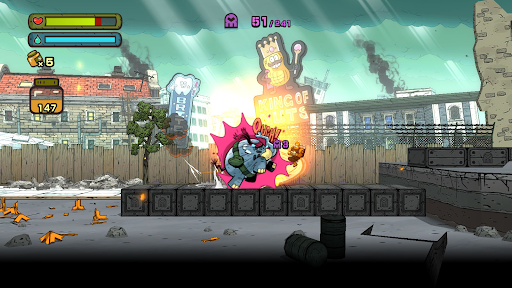
\includegraphics[width=\textwidth]{EjemploSemejanza.png}

%PRINCIPIO DE CONTINUIDAD
\item \textbf{Principio de Continuidad} \\
El ojo va a seguir siempre el camino visual más coherente y sencillo. Es atraído por la continuidad de una línea o una curva. Este principio puede ser usado para posicionar elementos parecidos en línea ya sean los coleccionables o las diferentes habilidades.\\
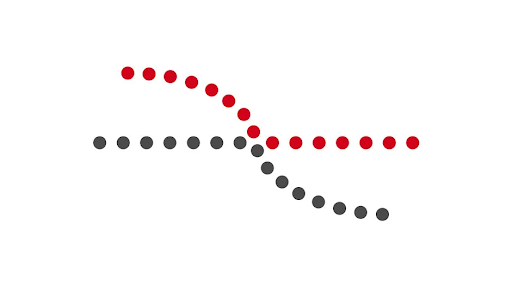
\includegraphics[width=\textwidth]{Imagenes/EjemploContinuidad.png}

%PRINCIPIO DE FIGURA Y FONDO
\item \textbf{Principio de Figura y Fondo} \\
La ambigüedad entre figura y fondo debe evitarse en los iconos de un videojuego para evitar distracciones o confusión en el jugador.\\
Ejemplo de ambigüedad:\\

\includegraphics[scale=0.4]{Imagenes/EjemploFiguraFondo.png}

%PRINCIPIO DE IGUALDAD
\item \textbf{Principio de Igualdad} \\
De  la misma manera en la que se debe evitar la ambigüedad entre figura y fondo en las imágenes que usemos, debemos evitar la confusión en una imagen que pueda parecer más de una cosa.\\

Ejemplo de ambigüedad: ¿Pato o conejo?\\
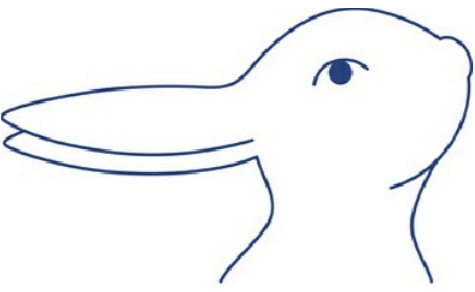
\includegraphics[width=\textwidth]{Imagenes/EjemploIgualdad.png}
Un ejemplo que da Celia Hodent en su libro Gamer 's Brain es que en el diseño de un juego FPS, en una imagen que representaba un radar, esta era reconocida por muchas personas como un trozo de pizza. Una vez desarrollada esta idea se hacía complicado ver el radar, así que fue modificada.

%PRINCIPIO DE SIMETRÍA
\item \textbf{Principio de simetría} \\
Este principio indica que elementos situados simétricamente o delimitados por unos límites simétricos son concebidos como un grupo.
Este principio puede ser aplicado en videojuegos para agrupar elementos relacionados entre sí.

%PRINCIPIO DE PROXIMIDAD
\item \textbf{Principio de proximidad} \\
Cuando varios ítems comparten una característica en común podemos agruparlas de forma próxima si la importancia es parecida  con el fin de que el usuario las perciba como que tienen un uso parecido.

Este principio puede ser muy útil a la hora de organizar elementos de la UI sin la necesidad de líneas para delimitar el espacio o flechas que sugieran una orientación.

\begin{itemize}
\item Interfaz en 2D\\
Los elementos que se pueden agrupar por proximidad son por una parte Vida y Escudos/Maana e Información del Personaje; por otra parte  Puntuación y Coleccionables;  como último Tiempo y Progreso del nivel.
\end{itemize}
\begin{itemize}
\item Interfaz en Shooter\\
Los elementos que se pueden agrupar por proximidad son Vida, Escudos y   Pociones.  Perteneciente a las armas tenemos la agrupación Munición, Equipamiento,  Armas y Habilidades.  Perteneciente al estado del juego se puede agrupar Puntos y Tiempo de Partida.
\end{itemize}

Un ejemplo de mal uso del principio de proximidad podría ser el árbol de habilidades de FarCry4, donde por proximidad, podría entenderse que el orden de mejora es por columnas, ya que cada ítem está más cerca del que tiene debajo que del que está a su lado. Sin embargo, el orden de mejora es por filas, de arriba a abajo y de izquierda a derecha.

Debajo se propone una mejora posible que podría acabar con la duda.

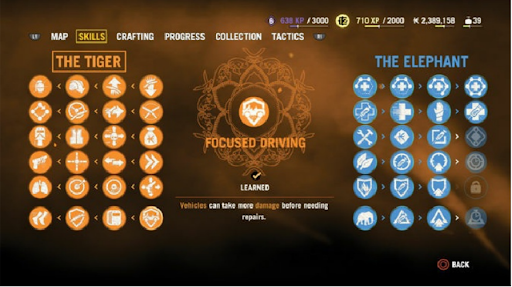
\includegraphics[width=\textwidth]{Imagenes/EjemploProximidad1.png}
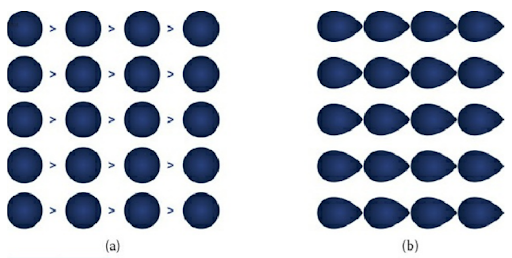
\includegraphics[width=\textwidth]{Imagenes/EjemploProximidad2.png}

%PRINCIPIO DE DIRECCIÓN COMÚN
\item \textbf{Principio de Dirección común} \\
Parecido al de continuidad los objetos que forman un patrón en la misma dirección son percibidos como parte de un grupo. Tiene el mismo uso que el de continuidad.
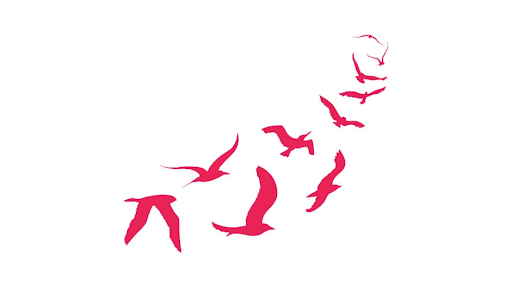
\includegraphics[width=\textwidth]{Imagenes/EjemploDireccionComun.png}

%OTROS PRINCIPIOS
\item \textbf{Otros principios}\\
Para otros principios como el de cierre, el de simplicidad o el de experiencia no hay aplicaciones claras y destacables al mundo de los videojuegos.
\end{itemize}
%%%%%%%%%%%%%%%%%%%%%%%%%%%%%%%%%%%%%%%%%%%%%%%%%%%%%%%%%%%%%%%%%%%%%%%%%%%%%%%%%%%%%%%%%%
% CBR
%%%%%%%%%%%%%%%%%%%%%%%%%%%%%%%%%%%%%%%%%%%%%%%%%%%%%%%%%%%%%%%%%%%%%%%%%%%%%%%%%%%%%%%%%
\subsection{Case Based Reasoning: que es, como funciona y aplicaciones}
%Que es ----
El CBR(Case-Based Reasoning)\cite{CBRLibro} es una forma de resolución de problemas basada en casos anteriores y conocidos. El caso(case) referencia a una experiencia o a un problema ya resuelto. Estos casos se pueden exponer de diferentes maneras. Los casos se componen de dos partes: el enunciado del problema y su solución. Una base de casos (case-base) será por tanto una colección de estos casos. El razonamiento significa que el enfoque tiene por objeto sacar conclusiones utilizando casos, dado un problema y formulando su solución.\\\\
El CBR es, en esencia, una técnica por la cual, a partir de un conocimiento previo (base de casos de la que se parte), donde encontramos problema-solución, podemos dado un problema, buscar la solución más cercana a ese problema y adaptarla. Una vez se adapte esta solución se añadirá a la base de casos con el fin de añadir este problema-solución.\\\\
%Formulación de un caso----
\textbf{Formulación de un caso}\\
En sistemas CBR podemos formular un caso de diferentes formas dependiendo de la formulación del problema o la comodidad del mismo caso. Así pues, un caso podría expresarse simplemente como una tupla <problema,solución> en sistemas poco complejos. También podríamos definirlos como valores asignados a los atributos que describen los casos. En la capa de la implementación esto puede ser un registro (si se usan bases de datos) o un objeto (si se usa programación orientada a objetos)\\\\
%Prblemas----
\textbf{Problemas}\\
Se crean a partir de una formulación previa en la que el usuario contesta, en el contexto del problema, sus atributos o sus prioridades ante dicha formulación. Por ejemplo en el caso de un coche con los atributos de color y precio, un problema podría ser la tupla <Rojo,10 000>\\\\
%Soluciones----
\textbf{Soluciones}\\
Las soluciones pueden ser de diferentes tipos desde un simple número hasta imágenes o explicaciones \\\\
%%%%%%%%%%%%%%% ETAPAS DEL CBR %%%%%%%%%%%%%%%%%%%
\textbf{Etapas del Case-Based Reasoning}\cite{CBR-UI}
\begin{itemize}
\item  Primero se comienza con una \textbf{descripción parcial del problema de entrada}, dado un usuario.
\end{itemize}
\begin{itemize}
\item  \textbf{Recuperación}
Se extrae de la base de casos los casos más \textbf{similares} o parecidos al dado. Estos casos se hallan a partir de una \textbf{función de similitud} la cual puede ser más o menos compleja. Los casos que se extraigan tienen que tener características en común con el problema que se quiere resolver. Después de realizar una búsqueda sobre el conjunto de casos, se hace un r\textbf{evaluación del conjunto de posibles soluciones} para hallar una más similar de manera más exhaustiva que la anterior.
\item \textbf{Reutilización}
Una vez se ha obtenido el caso más similar, existen dos formas de rehusar los casos: 
\begin{itemize}
\item  \textbf{Copiarlos} en caso de que su similitud sea igual o se perciba dentro de un rango impuesto por el sistema.
\item \textbf{Adaptarlos en caso contrario}. Para un uso sistemático de la adaptación se necesita un formalismo riguroso. Para este propósito, definimos los pasos de adaptación por reglas como acciones en general. Primero deberán de pasar una \textbf{precondición} para sí pueden ser adaptados o no. Tras esto, \textbf{se realizará una acción}:añadir o crear algo, eliminar algo, modificar algo: Este “algo” puede ser el valor de una variable, parte de la descripción de un objeto (subclase).s
\end{itemize}
\item \textbf{Revisión}
Es importante realizar una revisión por si la solución no es correcta, es decir, que las soluciones incorrectas también son introducidas en la base de conocimiento como ejemplo de errores con el fin de que el sistema no vuelva a tener los mismos errores .La evaluación de la solución se realiza aplicando la propia solución en el mundo real, es decir probando que sucedería si aplicaremos la solución obtenido en el contexto que se nos había producido el problema. Es evidente que la solución no tiene por qué probarse directamente sobre el mundo real, sino que este mundo puede simularse y recoger los datos que se obtienen de esta simulación. Una vez hecha esta evaluación hay que reparar los errores que pueda tener la solución.
\item  \textbf{Conservar/Aprender}
Una vez se tiene una solución revisada que satisface el problema, es importante añadirla a la base de casos con el fin de que nuestro sistema aprenda.
\end{itemize}

%%%%%%%%%%%%%%%%%%%%%%%%%%%%%%%%%%%%%%%%%%%%%%%%%%%%%%%%%%%%%%%%%%%%%%%%%%%%%%%%%%%%%%%%%%
%INVESTIGACION SOBRE ELEMENTOS
%%%%%%%%%%%%%%%%%%%%%%%%%%%%%%%%%%%%%%%%%%%%%%%%%%%%%%%%%%%%%%%%%%%%%%%%%%%%%%%%%%%%%%%%%
\subsection{Investigación sobre elementos comunes en interfaces de videojuegos}

Para entender y clasificar los atributos que comparten la mayoría de interfaces de videojuegos, extraímos los elementos más comunes de interfaces de varios juegos, dividiéndolos en dos grupos de acuerdo al género del juego. Dicha división dos géneros (Plataformas2D o First Person Shooter) viene dado porque las interfaces de los juegos que se incluyen en cada grupo comparten muchas propiedades y son más fáciles de clasificar dividiéndolos en estos dos grupos.
Tras escoger y analizar las interfaces de varios de ellos, volcamos la información en tablas donde podíamos consultar para cada juego si contiene cierto elemento en su interfaz y, en caso de tenerlo, las propiedades de dicho elemento en ese juego:\\\\
La posición del elemento indica su localización en el espacio de la interfaz. Permite distinguir entre elementos posicionados a los lados de la pantalla, si están centrados o no y su posición vertical.\\\\
La representación de cada elemento consiste en la forma en la que se representa en pantalla: desde un número hasta un icono o imagen para representar el atributo en cuestión.\\\\
En cuanto a la importancia del ítem, tomamos como importancia el valor que le da el usuario en pantalla al ítem en concreto, siendo más grande visualmente o menos dependiendo del valor gradual de la importancia. Esta importancia transcurre de muy poca importancia, poca importancia, media importancia, importante y muy importante. \\\\
El valor del atributo que se representa puede ser de tipo continuo o discreto. Esto es muy importante a la hora de definir el aspecto que tendrá dicho elemento en la interfaz porque hay representaciones más afines a valores continuos y otras a valores discretos. \\\\

\subsubsection{Plataforma 2D}

Para el género de Plataformas 2D fueron extraídos los siguientes elementos comunes en sus interfaces:
%%%%%%%%%%%%%%%%%%%%%%%%%%%%%%%%%%%%%%%%%%%%%%%%%%%%%%%%%%%%%%%%%%%%%%%%%%%%%%%%%%%%%%%%
%                               TABLA PLATAFORMA 2D                                    %
%%%%%%%%%%%%%%%%%%%%%%%%%%%%%%%%%%%%%%%%%%%%%%%%%%%%%%%%%%%%%%%%%%%%%%%%%%%%%%%%%%%%%%%%
\begin{table}
    \centering
            \begin{tabular}{|l|l|l|}
                \hline
            Atributo & Uso & Representación \\ 
                \hline
            %Tiempo------
            Tiempo & 
                \begin{tabular}[c]{@{}l@{}}Tiempo que ha pasado \\ desde el inicio (Cronómetro).\\ Cuenta atrás.
                \end{tabular} & 
                \begin{tabular}[c]{@{}l@{}}Barra (Discreta o continua).\\ Número.\\ Círculo.
                \end{tabular} \\ 
                \hline
            %Vida--------
            Vida
            & Puntos de vida restantes. &                                                                   
                \begin{tabular}[c]{@{}l@{}}Barra (Discreta o continua).\\ Círculo.\\ Símbolo.\\ Sectores.\\ Número.
                \end{tabular} \\ 
                \hline
            %Escudos----------
            Escudos & 
                \begin{tabular}[c]{@{}l@{}}Número de puntos de salud \\ complementarios a la vida.
                \end{tabular} &
                \begin{tabular}[c]{@{}l@{}}Barra.\\ Círculo.\\ Iconos.\\ Sectores.\\ Número.
                \end{tabular}\\ 
                \hline
            %Puntuación-------------
            Puntuación &
                \begin{tabular}[c]{@{}l@{}}Marcador de puntos \\conseguidos por el jugador
                \end{tabular}  &                                              
                \begin{tabular}[c]{@{}l@{}}Imagen o texto + Número.\\ Solo número.
                \end{tabular}\\ 
                \hline
            %Coleccionable---------
            Coleccionable &
                \begin{tabular}[c]{@{}l@{}}Número de objetos o ítems \\ recogidos a lo largo \\ del nivel / partida.
                \end{tabular} &
                \begin{tabular}[c]{@{}l@{}}Imagen o texto + Número.\\ 
                Solo número.
                \end{tabular}\\ 
                \hline
            %Progreso del personaje-----
                \begin{tabular}[c]{@{}l@{}}Progreso \\ del personaje
                \end{tabular} & 
                \begin{tabular}[c]{@{}l@{}}Representación del nivel \\ o  progreso del personaje \\ del juego.
                \end{tabular} & 
                \begin{tabular}[c]{@{}l@{}}Sectores.\\ Círculo.\\ Barra.\\ Número.
                \end{tabular}\\ 
                \hline
            Personaje & 
                \begin{tabular}[c]{@{}l@{}}Representación del \\ personaje en el \\juego en la interfaz 
                \end{tabular} &
                Imagen (Icono del personaje)\\ 
                \hline
            %Progreso del nivel-----
            Progreso del nivel &                          
                \begin{tabular}[c]{@{}l@{}}Indicación de la parte ya \\superada del nivel/partida
                \end{tabular} &
                \begin{tabular}[c]{@{}l@{}}Barra de progreso (Discreta \\ o continua).\\ Porcentaje.
                \end{tabular}\\ 
                \hline
            %Armas o habilidades-----
                \begin{tabular}[c]{@{}l@{}}Armas o \\ Habilidades
                \end{tabular}    & 
                \begin{tabular}[c]{@{}l@{}}Indicador de las armas o \\habilidades de las que \\dispone el jugador y su\\ número de usos.
                \end{tabular} & Imagen o texto + Número.\\
                \hline
            \end{tabular}

\end{table}

\subsubsection{First Person Shooter}
\subsubsection{Conclusiones}

